% Algebra 2 Lesson 2-3 fast-track packet: Factored Form of a Quadratic Function
% (enVision A2 2024 TE, Example 4 and Example 5 only; re-cut 2026-10-31 toward the Topic 2 test:
%  Topic Assessment items 4 and 7 are Example 4, item 14 is Example 5. No Practice block (R5: quiz
%  items 3 and 4 are rehearsed by Try Its 4 and 5). DOK 3 = Practice & Problem Solving 41 (Example 4),
%  the self-paced extension. Exit question = the TE's Additional Example 4, the parallel of topic item 4.)
% Shared preamble for the "fast" (hacked-down) Algebra 2 lesson packets, Oct 2026.
% Each packet: % Shared preamble for the "fast" (hacked-down) Algebra 2 lesson packets, Oct 2026.
% Each packet: % Shared preamble for the "fast" (hacked-down) Algebra 2 lesson packets, Oct 2026.
% Each packet: \input{fast-packet-template} then \begin{document} ... \end{document}.
\documentclass[12pt]{article}
\usepackage[margin=0.7in]{geometry}
\usepackage{amsmath,amssymb}
\usepackage{booktabs,tabularx,array}
\usepackage{enumitem}
\usepackage[T1]{fontenc}
\usepackage[utf8]{inputenc}
\usepackage{lmodern}
\usepackage{tikz}
\usepackage{pgfplots}
\pgfplotsset{compat=1.18}
\usepackage{xcolor}
\setlist{nosep,leftmargin=1.4em}
\setlength{\parindent}{0pt}
\setlength{\parskip}{6pt}
\renewcommand{\arraystretch}{1.35}
\newcolumntype{Y}{>{\raggedright\arraybackslash}X}
\pagestyle{empty}

% blanks and workspace
\newcommand{\blank}[1][2.6cm]{\rule[-2pt]{#1}{0.5pt}}
\newcommand{\lines}[1][1]{\par\vspace{2pt}\foreach \i in {1,...,#1}{\rule{0pt}{22pt}\rule{\linewidth}{0.4pt}\par}}
\newcommand{\wspart}[2]{\vspace{4pt}{\large\bfseries #1: #2}\par\vspace{-6pt}\rule{\textwidth}{0.4pt}\par}

% header: \packethead{Lesson 1-3}{Piecewise-Defined Functions}
\newcommand{\packethead}[2]{%
{\LARGE\bfseries #2}\hfill Name \blank[5cm]\\[2pt]
Algebra 2 \quad #1 (fast track) \hfill Date \blank[2.5cm] \quad Period \blank[1.2cm]\par\vspace{2pt}}

% boxed goals: \goals{learning goal}{language goal}
\newcommand{\goals}[2]{%
\fbox{\parbox{\dimexpr\textwidth-2\fboxsep-2\fboxrule}{%
\textbf{Learning goal:} #1\\[2pt]
\textbf{Language goal:} #2}}\par}

% quiz target box: \quiztarget{text}
\newcommand{\quiztarget}[1]{%
\vspace{4pt}\colorbox{gray!12}{\parbox{\dimexpr\textwidth-2\fboxsep}{\textbf{On the quiz:} #1}}\par}

% IXL table row helper: code & skill & which quiz question it feeds
\newcommand{\ixlrow}[3]{\texttt{#1} & #2 & #3 \\}

% one grid style for every graph; override xmin/xmax/... per plot
\pgfplotsset{sheetgrid/.style={
  axis lines=middle, grid=both, grid style={gray!45},
  xmin=-10.5, xmax=10.5, ymin=-10.5, ymax=10.5,
  xtick={-10,-8,...,10}, ytick={-10,-8,...,10},
  x=0.28cm, y=0.28cm,
  ticklabel style={font=\scriptsize, fill=white, inner sep=1pt},
  xlabel={$x$}, ylabel={$y$},
  axis line style={thick}, clip=true}}
% unit grid for small windows
\pgfplotsset{unitgrid/.style={sheetgrid,
  xmin=-5.5, xmax=5.5, ymin=-5.5, ymax=5.5,
  xtick={-5,...,5}, ytick={-5,...,5}, x=0.5cm, y=0.5cm}}
% open and closed endpoints
\tikzset{closed/.style={circle, fill, inner sep=1.6pt},
         open/.style={circle, draw, fill=white, inner sep=1.4pt}}
 then \begin{document} ... \end{document}.
\documentclass[12pt]{article}
\usepackage[margin=0.7in]{geometry}
\usepackage{amsmath,amssymb}
\usepackage{booktabs,tabularx,array}
\usepackage{enumitem}
\usepackage[T1]{fontenc}
\usepackage[utf8]{inputenc}
\usepackage{lmodern}
\usepackage{tikz}
\usepackage{pgfplots}
\pgfplotsset{compat=1.18}
\usepackage{xcolor}
\setlist{nosep,leftmargin=1.4em}
\setlength{\parindent}{0pt}
\setlength{\parskip}{6pt}
\renewcommand{\arraystretch}{1.35}
\newcolumntype{Y}{>{\raggedright\arraybackslash}X}
\pagestyle{empty}

% blanks and workspace
\newcommand{\blank}[1][2.6cm]{\rule[-2pt]{#1}{0.5pt}}
\newcommand{\lines}[1][1]{\par\vspace{2pt}\foreach \i in {1,...,#1}{\rule{0pt}{22pt}\rule{\linewidth}{0.4pt}\par}}
\newcommand{\wspart}[2]{\vspace{4pt}{\large\bfseries #1: #2}\par\vspace{-6pt}\rule{\textwidth}{0.4pt}\par}

% header: \packethead{Lesson 1-3}{Piecewise-Defined Functions}
\newcommand{\packethead}[2]{%
{\LARGE\bfseries #2}\hfill Name \blank[5cm]\\[2pt]
Algebra 2 \quad #1 (fast track) \hfill Date \blank[2.5cm] \quad Period \blank[1.2cm]\par\vspace{2pt}}

% boxed goals: \goals{learning goal}{language goal}
\newcommand{\goals}[2]{%
\fbox{\parbox{\dimexpr\textwidth-2\fboxsep-2\fboxrule}{%
\textbf{Learning goal:} #1\\[2pt]
\textbf{Language goal:} #2}}\par}

% quiz target box: \quiztarget{text}
\newcommand{\quiztarget}[1]{%
\vspace{4pt}\colorbox{gray!12}{\parbox{\dimexpr\textwidth-2\fboxsep}{\textbf{On the quiz:} #1}}\par}

% IXL table row helper: code & skill & which quiz question it feeds
\newcommand{\ixlrow}[3]{\texttt{#1} & #2 & #3 \\}

% one grid style for every graph; override xmin/xmax/... per plot
\pgfplotsset{sheetgrid/.style={
  axis lines=middle, grid=both, grid style={gray!45},
  xmin=-10.5, xmax=10.5, ymin=-10.5, ymax=10.5,
  xtick={-10,-8,...,10}, ytick={-10,-8,...,10},
  x=0.28cm, y=0.28cm,
  ticklabel style={font=\scriptsize, fill=white, inner sep=1pt},
  xlabel={$x$}, ylabel={$y$},
  axis line style={thick}, clip=true}}
% unit grid for small windows
\pgfplotsset{unitgrid/.style={sheetgrid,
  xmin=-5.5, xmax=5.5, ymin=-5.5, ymax=5.5,
  xtick={-5,...,5}, ytick={-5,...,5}, x=0.5cm, y=0.5cm}}
% open and closed endpoints
\tikzset{closed/.style={circle, fill, inner sep=1.6pt},
         open/.style={circle, draw, fill=white, inner sep=1.4pt}}
 then \begin{document} ... \end{document}.
\documentclass[12pt]{article}
\usepackage[margin=0.7in]{geometry}
\usepackage{amsmath,amssymb}
\usepackage{booktabs,tabularx,array}
\usepackage{enumitem}
\usepackage[T1]{fontenc}
\usepackage[utf8]{inputenc}
\usepackage{lmodern}
\usepackage{tikz}
\usepackage{pgfplots}
\pgfplotsset{compat=1.18}
\usepackage{xcolor}
\setlist{nosep,leftmargin=1.4em}
\setlength{\parindent}{0pt}
\setlength{\parskip}{6pt}
\renewcommand{\arraystretch}{1.35}
\newcolumntype{Y}{>{\raggedright\arraybackslash}X}
\pagestyle{empty}

% blanks and workspace
\newcommand{\blank}[1][2.6cm]{\rule[-2pt]{#1}{0.5pt}}
\newcommand{\lines}[1][1]{\par\vspace{2pt}\foreach \i in {1,...,#1}{\rule{0pt}{22pt}\rule{\linewidth}{0.4pt}\par}}
\newcommand{\wspart}[2]{\vspace{4pt}{\large\bfseries #1: #2}\par\vspace{-6pt}\rule{\textwidth}{0.4pt}\par}

% header: \packethead{Lesson 1-3}{Piecewise-Defined Functions}
\newcommand{\packethead}[2]{%
{\LARGE\bfseries #2}\hfill Name \blank[5cm]\\[2pt]
Algebra 2 \quad #1 (fast track) \hfill Date \blank[2.5cm] \quad Period \blank[1.2cm]\par\vspace{2pt}}

% boxed goals: \goals{learning goal}{language goal}
\newcommand{\goals}[2]{%
\fbox{\parbox{\dimexpr\textwidth-2\fboxsep-2\fboxrule}{%
\textbf{Learning goal:} #1\\[2pt]
\textbf{Language goal:} #2}}\par}

% quiz target box: \quiztarget{text}
\newcommand{\quiztarget}[1]{%
\vspace{4pt}\colorbox{gray!12}{\parbox{\dimexpr\textwidth-2\fboxsep}{\textbf{On the quiz:} #1}}\par}

% IXL table row helper: code & skill & which quiz question it feeds
\newcommand{\ixlrow}[3]{\texttt{#1} & #2 & #3 \\}

% one grid style for every graph; override xmin/xmax/... per plot
\pgfplotsset{sheetgrid/.style={
  axis lines=middle, grid=both, grid style={gray!45},
  xmin=-10.5, xmax=10.5, ymin=-10.5, ymax=10.5,
  xtick={-10,-8,...,10}, ytick={-10,-8,...,10},
  x=0.28cm, y=0.28cm,
  ticklabel style={font=\scriptsize, fill=white, inner sep=1pt},
  xlabel={$x$}, ylabel={$y$},
  axis line style={thick}, clip=true}}
% unit grid for small windows
\pgfplotsset{unitgrid/.style={sheetgrid,
  xmin=-5.5, xmax=5.5, ymin=-5.5, ymax=5.5,
  xtick={-5,...,5}, ytick={-5,...,5}, x=0.5cm, y=0.5cm}}
% open and closed endpoints
\tikzset{closed/.style={circle, fill, inner sep=1.6pt},
         open/.style={circle, draw, fill=white, inner sep=1.4pt}}

\newcommand{\twolines}[1][1]{\par\vspace{2pt}\foreach \i in {1,...,#1}{\rule{0pt}{22pt}\rule{0.48\textwidth}{0.4pt}\hfill\rule{0.48\textwidth}{0.4pt}\par}}
\begin{document}

\packethead{Lesson 2-3}{Factored Form of a Quadratic Function}
\goals{I can find the zeros of a quadratic function by factoring, use them to answer a real-world question, and use them to find where the function is positive or negative.}{I can explain what the zeros of a function tell me using the words \emph{factor}, \emph{zero}, \emph{Zero Product Property}, \emph{x-intercept}, and \emph{interval}.}

\quiztarget{You will (1) factor $3x^2-11x-4$ (full Savvas quiz only); (2) solve $x^2+7x=30$ by factoring, the steps of Examples 4 and 5; (3) find when a launched object lands (Example 4, Try It 4; bonus); (4) find where a quadratic function is positive (Example 5, Try It 5); (5) write a long-jumper's parabola (full Savvas quiz only).}
\topictarget{2}{Question 4 asks for a rectangle's width from its area (Example 4; the Exit question is the same kind). Question 7 asks when a ball thrown from a stadium hits the ground (Example 4). Question 14 asks when a launched ball is higher than 12\,m, an inequality (Example 5; you also need the Quadratic Formula from Lesson 2-6).}

\textbf{Zero Product Property:} if $ab=0$, then $a=0$ or $b=0$ (or both). To use it, rewrite the equation so one side is $0$, factor, then set each \textbf{factor} equal to $0$. \hfill {\small Spanish: \emph{Propiedad del cero del producto}; zero of a function = \emph{cero de una función}.}

\wspart{Example 4}{Find the Zeros of a Quadratic Function}
A multilevel driving range has three levels. Marco hits golf balls from the second level, which is 32\,ft high. The height of a ball at $x$ seconds after Marco hits it is modeled by the function $h(x)=-16x^2+16x+32$. When does the ball hit the ground?

\begin{minipage}[t]{0.53\textwidth}
\vspace{0pt}
\begin{enumerate}[label=\textbf{\arabic*.}, itemsep=2pt]
\item The ball hits the ground when the height, $h(x)$, is $0$:\\ $0=-16x^2+16x+32$
\item Factor out the GCF, $-16$:\\ $0=-16(x^2-x-2)$
\item Factor. Be careful of the signs: two numbers with product $-2$ and sum $-1$ are $1$ and $-2$.\\ $0=-16(x+1)(x-2)$
\item Zero Product Property ($-16$ is never $0$):\\ $x+1=0$ \ or \ $x-2=0$, so $x=-1$ \ or \ $x=2$
\end{enumerate}
\end{minipage}\hfill
\begin{minipage}[t]{0.43\textwidth}
\vspace{0pt}\raggedright
The \textbf{zeros} of the function are at $x=-1$ and $x=2$. They are the solutions of $0=-16x^2+16x+32$ and the \textbf{x-intercepts} of the graph of $h$.

\textbf{Which zero makes sense?} Time has to be positive, so $x=2$ is the only solution that makes sense. After \textbf{2 seconds}, the golf ball hits the ground.

\textbf{Check:} $h(2)=-16(4)+16(2)+32$\\ \phantom{\textbf{Check:} }${}=-64+32+32=0$ \checkmark
\end{minipage}

\vspace{2pt}
\textbf{Say it:} After I \emph{factor}, the \emph{zeros} of $h$ are \blank[1.2cm] and \blank[1.2cm], by the \emph{Zero Product Property}. They are the \emph{x-intercepts} of the graph. The ball hits the ground after \blank[1.2cm] seconds, not \blank[1.2cm] seconds, because \dots
\lines[2]

\newpage
\wspart{Try It 4}{When does the ball reach the ground?}
A baseball is thrown from the upper deck of a stadium, 128\,ft above the ground. The function $h(x)=-16x^2+32x+128$ gives the height of the ball $x$ seconds after it is thrown. How long will it take the ball to reach the ground?

\begin{minipage}[t]{0.55\textwidth}
\vspace{0pt}\raggedright
Set the height equal to $0$: \quad $0=\blank[3.6cm]$\par\vspace{8pt}
Factor out the GCF: \quad $0=-16\,(\blank[2.8cm])$\par\vspace{8pt}
Factor: \quad $0=-16\,(\blank[1.6cm])(\blank[1.6cm])$\par\vspace{8pt}
Zeros: \quad $x=\blank[1.2cm]$ \ or \ $x=\blank[1.2cm]$
\end{minipage}\hfill
\begin{minipage}[t]{0.41\textwidth}
\vspace{0pt}\raggedright
Which zero makes sense? Why?
\lines[3]
The ball reaches the ground after \blank[1.4cm] seconds.
\end{minipage}

% R3: the lesson's DOK 3 is Practice & Problem Solving 41 (Use Structure, the drone), filed under
% Example 4 in the TE item analysis; 39, 45 and 10 are Example 6 (cut). Self-paced extension.
\wspart{Extension (DOK 3)}{Drone flight (Practice \& Problem Solving 41)}
\textbf{Use Structure} A drone leaves its launch pad, flies down over the edge of a cliff, and then it flies back up again. The ordered pairs are the drone's flight time and height:\quad $(0\text{ s},\,5\text{ m})$,\quad $(5\text{ s},\,0\text{ m})$,\quad $(10\text{ s},\,0\text{ m})$,\quad $(15\text{ s},\,5\text{ m})$.

\textbf{a.} What does each point represent for the drone and its height?
\lines[2]

\textbf{b.} Write a function that represents the drone's height with respect to time. Factor your function if it is factorable.

Hint: the \emph{zeros} are $5$ and $10$, so $h(x)=a(x-5)(x-10)$. Substitute the point $(0,5)$ to find $a$.
\twolines[2]
$h(x)=\blank[4.5cm]$

\textbf{c.} How far below the platform does the drone fly? \qquad \textbf{d.} How could you validate this model?
\twolines[3]

\newpage
\wspart{Example 5}{Determine Positive or Negative Intervals}
Identify the interval(s) on which the function $y=x^2-2x-3$ is positive.

\begin{minipage}[t]{0.57\textwidth}
\vspace{0pt}\raggedright
The $y$-values of a quadratic function can only turn from positive to negative or from negative to positive when the graph crosses the $x$-axis. Find the \textbf{zeros} to find these points.

$0=x^2-2x-3$\\
$0=(x-3)(x+1)$\\
$x-3=0$ \ or \ $x+1=0$\\
$x=3$ \ or \ $x=-1$

Two zeros create three \textbf{intervals}. Choose an $x$-value to test in each interval.
\end{minipage}\hfill
\begin{minipage}[t]{0.4\textwidth}
\vspace{0pt}\centering
\begin{tikzpicture}
\begin{axis}[unitgrid, x=0.5cm, y=0.5cm,
  xtick={-4,-2,2,4}, ytick={-4,2,4},
  minor xtick={-5,...,5}, minor ytick={-5,...,5},
  every axis x label/.style={at={(current axis.right of origin)}, anchor=north west}]
\addplot[thick, red, domain=-2:4, samples=80, <->] {x^2-2*x-3};
\node[closed, red] at (axis cs:-1,0) {};
\node[closed, red] at (axis cs:3,0) {};
\node[closed, red] at (axis cs:0,-3) {};
\node[font=\scriptsize, fill=white, inner sep=1pt, anchor=south east] at (axis cs:-1.35,0.25) {$(-1,0)$};
\node[font=\scriptsize, fill=white, inner sep=1pt, anchor=south west] at (axis cs:3.35,0.25) {$(3,0)$};
\node[font=\scriptsize, fill=white, inner sep=1pt, anchor=west] at (axis cs:0.15,-3) {$-3$};
\node[font=\scriptsize, fill=white, inner sep=1pt, anchor=north east] at (axis cs:-0.05,-0.05) {$O$};
\node[font=\scriptsize, red, fill=white, inner sep=1pt, anchor=south east] at (axis cs:5.3,-5.3) {$y=x^2-2x-3$};
\end{axis}
\end{tikzpicture}
\end{minipage}

\vspace{2pt}
\begin{tabularx}{\textwidth}{Y Y Y}
\toprule
$x<-1$ & $-1<x<3$ & $x>3$ \\
Choose $x=-3$. & Choose $x=1$. & Choose $x=6$. \\
$y=(-3)^2-2(-3)-3$ & $y=(1)^2-2(1)-3$ & $y=(6)^2-2(6)-3$ \\
${}=9+6-3=12$ & ${}=1-2-3=-4$ & ${}=36-12-3=21$ \\
\textbf{Positive} & \textbf{Negative} & \textbf{Positive} \\
\bottomrule
\end{tabularx}

The function is positive when the graph is above the $x$-axis, on the intervals $(-\infty,-1)$ and $(3,\infty)$.

\textbf{Say it:} I \emph{factor} to find the \emph{zeros} \blank[1.2cm] and \blank[1.2cm]. They are the \emph{x-intercepts}, and they cut the $x$-axis into three \emph{intervals}. The function is positive on \blank[3cm] because \dots
\lines[2]

\wspart{Try It 5}{Where is the function negative?}
Identify the interval(s) on which the function $y=x^2-4x-21$ is negative.

Factor: \quad $0=(\blank[1.6cm])(\blank[1.6cm])$ \qquad Zeros: \quad $x=\blank[1.2cm]$ \ and \ $x=\blank[1.2cm]$

\renewcommand{\arraystretch}{1.6}
\begin{tabularx}{\textwidth}{l Y Y Y}
\toprule
Interval & \blank[2.4cm] & \blank[2.4cm] & \blank[2.4cm] \\
Test $x$ & & & \\
$y$ & & & \\
Sign & & & \\
\bottomrule
\end{tabularx}
\renewcommand{\arraystretch}{1.35}

The function is negative on the interval \blank[4cm].

\newpage
\wspart{IXL}{Practice for the quiz}
Go to IXL, Algebra 2. Type the code in the search box. Do the starred skills first.
\textbf{SmartScore 70 or above on each starred ($\bigstar$) skill replaces your quiz score.}

\vspace{2pt}
\begin{tabularx}{\textwidth}{l Y Y}
\toprule
\textbf{Code} & \textbf{Skill} & \textbf{Feeds} \\
\midrule
\ixlrow{TRU}{Solve a quadratic equation using the zero product property}{Warm-up for Example 4 (optional): the factors are already given}
\ixlrow{NMZ $\bigstar$}{Factor out a monomial}{Quiz 3 (bonus): the $-16$ step of Example 4 and Try It 4}
\ixlrow{CJC $\bigstar$}{Solve a quadratic equation by factoring}{Quiz 2 and Quiz 3: Example 4 and Try It 4}
\ixlrow{DP9 $\bigstar$}{Graph solutions to quadratic inequalities}{Quiz 4: Example 5 and Try It 5}
\ixlrow{UB5}{Factor quadratics}{Quiz 1 (full Savvas quiz only): factor $ax^2+bx+c$}
\midrule
\multicolumn{3}{@{}l@{}}{\parbox{\textwidth}{\small\raggedright Optional, not on the short form: \texttt{G2Q} Write a quadratic function from its zeros and \texttt{HPB} Write a quadratic function in factored form from its x-intercepts and another point (Quiz 5, full Savvas quiz only; also the drone extension).\strut}} \\
\bottomrule
\end{tabularx}

\textbf{Before the quiz, finish these sentences.}

To find when a launched object hits the ground, I set $h(x)$ equal to \blank[1.5cm], \emph{factor}, and use the \emph{Zero Product Property}. If $0=-16(x+2)(x-5)$, then $x=\blank[1.2cm]$ or $x=\blank[1.2cm]$; in a time problem I keep only \blank[1.2cm].

Each \emph{zero} of a quadratic function is an \emph{x-intercept} of its graph because
\lines[1]

Two zeros cut the $x$-axis into \blank[1.2cm] \emph{intervals}. To tell whether the function is positive on an interval, I
\lines[1]

% Exit: the TE's Additional Example 4 (for Example 4), the parallel of Topic 2 test item 4 (rectangle, area, length longer than width).
% The TE's printed second line w^2 - 5w = 50 is a slip for w^2 + 5w = 50 (not shown to students). Key: w(w+5) = 50,
% w^2 + 5w - 50 = 0, (w+10)(w-5) = 0, w = 5 (w = -10 rejected): 5 in. by 10 in.
\vspace{2pt}
\fbox{\parbox{\dimexpr\textwidth-2\fboxsep-2\fboxrule}{%
\begin{minipage}[t]{0.6\linewidth}\vspace{0pt}\raggedright
\textbf{Exit question.} The length of a rectangle is 5\,in. longer than its width and the rectangle has an area of $50\text{ in.}^2$. What are the dimensions of the rectangle? Without graphing, how do you know which \emph{zero} is a possible solution?
\end{minipage}\hfill
\begin{minipage}[t]{0.36\linewidth}\vspace{0pt}\centering
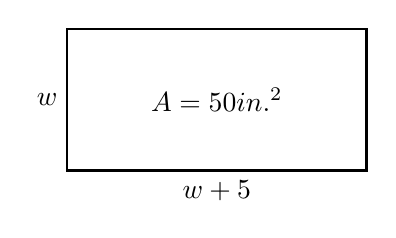
\begin{tikzpicture}
\draw[thick] (0,0) rectangle (3.8,1.8);
\node[left] at (0,0.9) {$w$};
\node[below] at (1.9,0) {$w+5$};
\node at (1.9,0.9) {$A=50\text{ in.}^2$};
\end{tikzpicture}
\end{minipage}
\lines[3]\vspace{4pt}}}

\end{document}
